%  !TeX  root  =  user_guide.tex

\chapter{QGIS Server}\label{label_qgisserver}
\index{WMS!QGIS Server}

% when the revision of a section has been finalized,
% comment out the following line:
% \updatedisclaimer

QGIS Server ist eine Open Source Implementierung des WMS 1.3, die zus�tzliche 
kartographische Funktionen f�r thematische Karten zur Verf�gung stellt. Der QGIS
Server ist eine FastCGI/CGI (Common Gateway Interface)-Anwendung, ist in C++ 
geschrieben und arbeitet mit einem Webserver zusammen (z.B. Apache oder Lighttpd). 
Es wurde mit finanziellen Mitteln des EU Projekts Orchestra, Sany und der 
Satdt Uster aus der Schweiz entwickelt. 

QGIS Server verwendet QGIS im Hintergrund f�r die GIS-Logik und f�r das Darstellen 
der Karte. Weiterhin wird die Qt-Bibliothek f�r Grafiken und f�r die 
plattformunabh�ngige C++-Programmierung verwendet. Im Gegensatz zu anderer 
WMS-Software verwendet der QGIS Server kartographische Regeln in SLD/SE als 
Konfigurationssprache, sowohl f�r die Server Konfiguration als auch f�r die 
benutzerdefinierten kartographischen Regeln.

Dar�ber hinaus bietet das QGIS Server Projekt ein 'Publish to Web' Plugin. 
Dies ist ein Plugin f�r den QGIS-Desktop, welches die aktuellen Layer und ihre 
Darstellung als Web-Projekt f�r den QGIS Server (mit kartographischen 
Visualisierung Regeln ausgedr�ckt in SLD) exportiert.

Da QGIS Desktop und QGIS Server die gleichen Bibliotheken f�r die 
Visualisierung verwenden, sehen die Karten, die im Web ver�ffentlicht werden, 
genauso aus wie im Kartenfenster des Desktop-GIS. Das Plugin unterst�tzt derzeit 
grundlegenden Symbolisierung. Komplexere kartographischen Visualisierungsregeln 
m�ssen noch manuell erg�nzt werden. Da die Konfiguration ausschlie�lich auf dem 
SLD-Standard beruht und seine Erweiterungen gut dokumentiert sind, muss man nur
eine standardisierte Sprache lernen. Dies vereinfacht die Komplexit�t der 
Erstellung von Karten f�r das Web enorm.

In den folgenden Handb�chern werden wir dieses Thema noch ausweiten. Bis dahin 
empfehlen wir Ihnen die folgenden Internetseiten f�r weitere Informationen:

\url{http://karlinapp.ethz.ch/qgis\_wms/} \\
\url{http://www.qgis.org/wiki/QGIS\_Server\_tutorial} \\
\url{http://linfiniti.com/2010/08/qgis-Server-a-wms-server-for-the-masses/}

\section{Beispielinstallation unter Debian Squeeze}

An dieser Stelle wollen wir eine kurze und einfache Installationsanleitung f�r 
das GNU/Linux Debian Squeeze geben. Viele andere OS bieten auch fertige Pakete 
f�r den QGIS Server. Wenn Sie alles aus dem Quellcode erstellen wollen, lesen 
Sie bitte die URLs oben.

Abgesehen von QGIS Desktop und QGIS Server ben�tigen Sie einen Webserver, in 
unserem Fall apache2. Sie k�nnen alle Pakete mit aptitude oder apt-get install 
zusammen installieren. Alle weiteren notwendigen Pakete werden dann mitinstalliert.

Nach der Installation sollten Sie testen, ob der Webserver und der QGIS Server 
wie erwartet funktionieren.

Vergewissern Sie sich, dass der Apache Webserver l�uft. Ansonsten starten Sie ihn 
mit '/etc/init.d/apache2 start'. �ffen Sie nun einen Web-Browser und geben Sie sie 
URL http://localhost ein. Wenn alles in Ordnung ist, sollten Sie die Meldung 'It 
works' sehen.

Jetzt testen wir die QGIS Server Installation. Die Datei qgis\_mapserv.fcgi finden Sie 
unter /usr/lib/cgi-bin/qgis\_mapserv.fcgi und stellt einen Test-WMS bereit, der die Staatsgrenzen der Vereinigten Staaten von Amerika zeigt \ref{fig:usa_wms}. Laden Sie 
den WMS mit der URL http://localhost/cgi-bin/qgis\_mapserv.fcgi wie in Abschnitt \ref{sec:ogc-wms-layers} beschrieben.

\begin{figure}[ht]
\centering
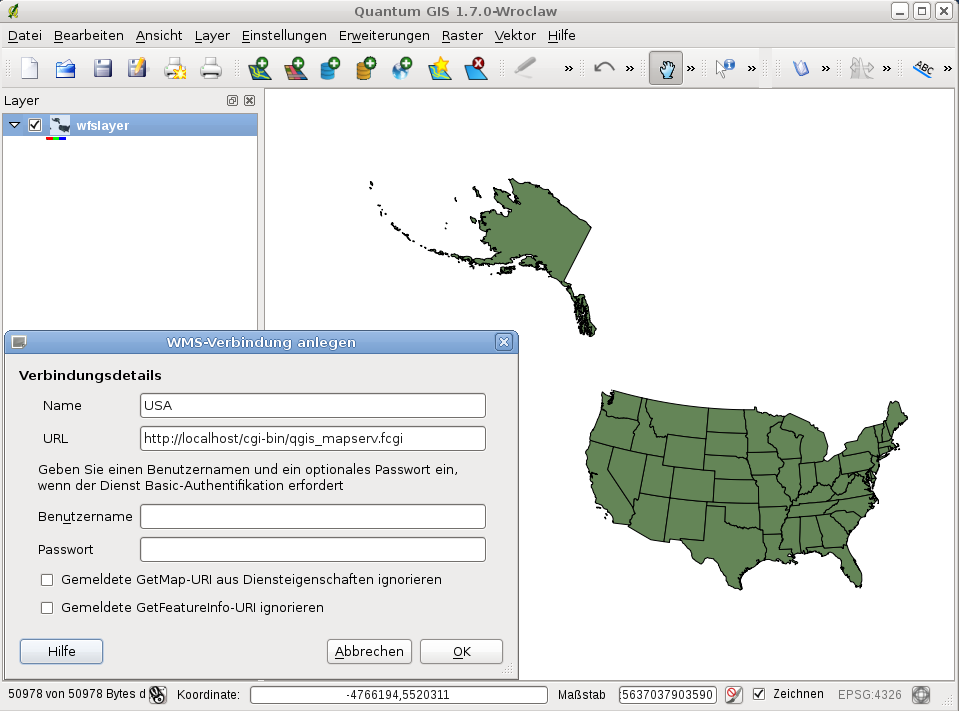
\includegraphics[clip=true, width=14cm]{standard_wms_usa}
\caption{Standard QGIS Server WMS mit Grenzen der USA \nixcaption}
\label{fig:usa_wms}
\end{figure}

\section{Erstellen eines WMS aus einem QGIS Projekt}

Um einen neuen QGIS WMS Server zu erstellen, brauchen wir eine QGIS Projekt-Datei 
mit einigen Layern. Hier verwenden wir die 'regions' und 'airports' Shapefiles 
aus dem QGIS Beispieldatensatz.

Laden Sie zun�chst die Shapefiles und definieren Sie die Farben und Stile der Layer 
und das KBS in QGIS, wenn nicht bereits geschehen ist. Im n�chsten Schritt �ffnen 
Sie den \tab{WMS Server} Reiter im Men� \mainmenuopt{Einstellungen} \arrow 
\mainmenuopt{Projekteigenschaften} und definieren Sie die Felder 
'Diensteigenschaften', 'Koordinatensystemeinschr�nkungen' und 'Angezeigt Ausmasse'. Zus�tzlich k�nnen Sie das Kontrollk�stchen \checkbox{WKT-Geometrien in 
Objektinformationen einschliessen} aktivieren, um die Layer abfragbar zu machen 
(siehe Abbildung \ref{fig:wmsdefinition}). Speichern Sie nun die Sitzung als 
Projekt-Datei 'alaska\_airports.qgs'.

\begin{figure}[ht]
\centering
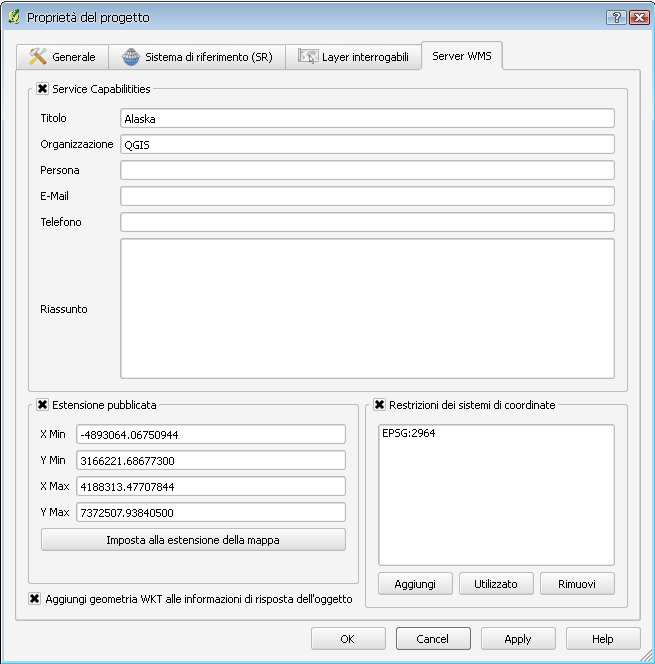
\includegraphics[clip=true, width=9cm]{wms_server_definition}
\caption{Definitionen f�r einen QGIS Projekt WMS Server \nixcaption}
\label{fig:wmsdefinition}
\end{figure}

Um das Projekt als WMS bereitzustellen, erstellen Sie einen neuen Ordner 
'/usr/lib/cgi-bin/project' mit Admin-Rechten und f�gen Sie die Projekt-Datei 
'alaska\_airports.qgs' und eine Kopie der qgis\_mapserv.fcgi Datei hinzu. 
Das ist alles.

Nun testen wir den Projekt WMS. Laden Sie den WMS mit der URL 
'http://localhost/cgi-bin/project/qgis\_mapserv.fcgi' wie in Abschnitt 
\ref{sec:ogc-wms-servers} beschrieben in QGIS. Siehe Abbildung \ref{fig:wmsproject}.

\begin{figure}[ht]
\centering
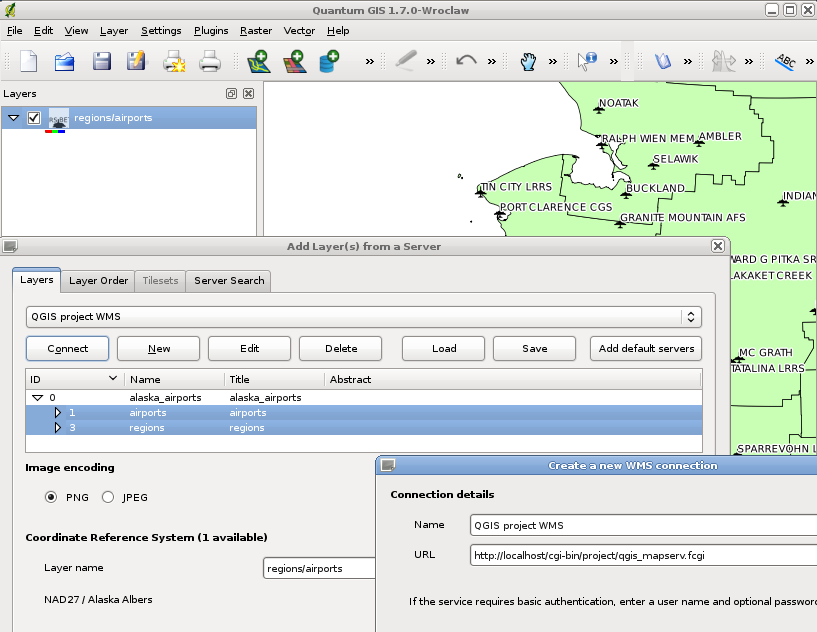
\includegraphics[clip=true, width=\textwidth]{wms_server_project}
\caption{QGIS WMS Server basierend auf einem QGIS Projekt \nixcaption}
\label{fig:wmsproject}
\end{figure}

\FloatBarrier
